%!TEX root = ../masters_thesis.tex

\chapter{Basics} % (fold)
\label{cha:basics}

According to the title of this Master's Thesis:

\vspace{-1em}
\begin{large}
\begin{center}
  \textbf{
    \emph{Visualizing}$^1$ and \emph{Editing}$^2$ the \emph{History}$^3$ of\\
    \emph{Countries}$^4$ in \emph{Time and Space}$^5$ with \emph{HistoGlobe}$^6$
  }
\end{center}
\end{large}
\vspace{-1em}

this chapter will form the theoretical foundation and present related work:

\begin{description}[labelindent=1.53em]
  \item[$^1$] The purpose of a \emph{visualization} is to visually present information to a human in a comprehensible way. The visualization is one component of an \emph{Historical Geographic Information System} introduced in section \ref{sec:historical_geographic_information_systems}.
  \item[$^2$] An information system can allow the user to modify, correct or generally \emph{edit} the information in the system.
  \item[$^3$] History is the study of our past, to understand the present and reason about the future. Its main ideas are introduced in section \ref{sub:history_vs_geography}.
  \item[$^4$] A \emph{country} is commonly referred to as a political entity with a clearly defined territory, a permanent population and a government. But as section \ref{sec:countries} shows, its definition is surprisingly difficult.
  \item[$^5$] The work in this thesis focuses on data models of \emph{time and space}. Existing \emph{spatio-temporal data models} are discussed in section \ref{sec:spatio_temporal_data_models}.
  \item[$^6$] The chapter closes in \ref{sec:histoglobe} with a presentation of \emph{HistoGlobe}, a web-based HGIS that was used to implement the data model developed in this thesis.
\end{description}

% ==============================================================================
\section{Countries} % (fold)
\label{sec:countries}

Almost everybody in the world is familiar with the term ``country'', because almost everybody has at least one home country he or she can potentially hold a passport from. However, the reality is very complex. If the information system of this thesis deals with countries, it must be possible to decide for each current and historic political entity in the world if it is or was a country or not. This requires a clear and non-conflicting definition of a country. This section will show that this is impossible.

The Oxford English Dictionary reads as follows: ``The \emph{territory} of a \emph{nation}; a \emph{region} constituting an \emph{independent state}, or a region, province, etc., which was once independent and is still distinct in institutions, language, etc.'' \cite{oxendict}.
This definition includes many different concepts and terms: the territory or region that the country is on, a nation or state, a population and a culture of the territory in terms of institutions or languages. \emph{Nation} and \emph{state} are commonly used as synonyms for countries.

To understand what a country really is, it is helpful to consult the United Nations, an intergovernmental organization that was founded in October 1945. It promotes international peace keeping, security and protection of human rights. The committee currently has 193 full member states and two permanent observers\cite{UNmembers}. But these 195 members do not cover all places in the world -- and also a membership in the United Nations does not guarantee being an undisputed country.

% ------------------------------------------------------------------------------
\subsection{Problematic Cases} % (fold)
\label{sub:special_cases}

Examining the list of the UN member states yields several special cases, which can be classified by their membership status in the United Nations and their degree of international recognition.


% - - - - - - - - - - - - - - - - - - - - - - - - - - - - - - - - - - - - - - -
\paragraph{UN observer states} % (fold)
\label{par:un_observer_states}

The \emph{Holy See} is the juridical and spiritual entity representing Vatican City. It is a fully recognized and sovereign state but not a full member of the UN, because it has never applied. It is by far the smallest sovereign state in the world (0.44 km²), an enclave inside the city of Rome with a population of only 800 people \cite{VaticanPopulation}.

The \emph{State of Palestine} with a population of 4.8 million people as of 2016 \cite{PalestinePopulation} has a totally different situation, because it does not have a clearly defined territory. The West Bank, East Jerusalem and the Gaza Strip were created in the 1949 Green Line Armistice Agreement, but were never intended to be used as international boundaries \cite{PalestineTerritory}. Moreover, while 114 states officially recognize the Palestinian state, almost all current main economic powers do not, including Germany and the United States. Unlike the Holy See, Palestine is not a fully sovereign and recognized country.

% paragraph un_observer_states (end)

% - - - - - - - - - - - - - - - - - - - - - - - - - - - - - - - - - - - - - - -
\paragraph{UN non-members with limited recognition} % (fold)
\label{par:un_non_members_with_limited_recognition}

\emph{Kosovo} declared independence from Serbia in 2008. It has a clearly defined territory and a permanent population and is recognized by 111 UN member states. In order for Kosovo to become a full member of the United Nations, all permanent members of the security council (United Kingdom, France, Russia, China and the United States) must agree. But since Russia and China strongly support the territorial integrity of Serbia, they would veto Kosovo's membership. Therefore, Kosovo is not even a UN observer state, although it has about the same degree of international recognition as Palestine \cite{KosovoThanksYou}.

The status of \emph{Taiwan} is a very complicated issue. Two territories and two political entities are involved in the conflict: the \emph{People's Republic of China}, commonly known as China, has full control over mainland China, and the \emph{Republic of China} governs the island of Taiwan. The problem is that both states claim the exact same territory: mainland China and the island of Taiway. Since 1971 the People's Republic of China is the only representative of whole China in the United Nations, including Taiwan. It is part of the Security Council and can successfully veto membership requests of the Republic of China. However, Taiwan operates like an independent country by international standards. They have their own jurisdiction, issue their own passports and have unofficial diplomatic relations to most countries in the world. Only 22 UN members officially uphold diplomatic relations to Taiwan \cite{TaiwanRecognition}. To all of these states the People's Republic of China does not kepp any diplomatic relations.

There are other places with limited international recognition: the Sahrawi Arab Democratic Republic (recognized by 84 UN member states) \cite{WesternSaharaRecognition}, Abkhazia (6) \cite{AbkhaziaRecognition}, South Ossetia (5) \cite{SouthOssetiaRecognition}, the Turkish Republic of Northern Cyprus (1) \cite{NorthernCyprusRecognition}, Nagorno-Karabakh Republic (0) \cite{NagornoRecognition}, Transnistria (0) \cite{TransnistriaRecognition} and Somaliland (0) \cite{SomalilandRecognition}.

% paragraph un_non_members_with_limited_recognition (end)

% - - - - - - - - - - - - - - - - - - - - - - - - - - - - - - - - - - - - - - -
\paragraph{UN members with limited recognition} % (fold)
\label{par:un_members_with_limited_recognition}

In addition to the Republic of China, there are five other member states of the United Nations that are not fully recognized by all other UN members: Armenia is not recognized by Pakistan \cite{ArmeniaRecognition}, Turkey does not recognize the Republic of Cyprus \cite{CyprusRecognition}, North and South Korea mutually do not recognize each other \cite{KoreaRecognition} and the State of Israel is not recognized by 32 UN member states \cite{IsraelRecognition}.

% paragraph un_members_with_limited_recognition (end)

% - - - - - - - - - - - - - - - - - - - - - - - - - - - - - - - - - - - - - - -
\paragraph{Special Territories} % (fold)
\label{par:special_territories}

There are also territories belonging to fully sovereign countries with a varying degree of sovereignty: Greenland is an autonomous country within the Kingdom of Denmark, but not a sovereign state. The same applies to numerous overseas territories of the United Kingdom, the French Republic or the Kingdom of the Netherlands. Moreover, there are five quasi-independent countries in a so called \emph{Free Association}: Niue and Cook Islands are associated to New Zealand and not part of the United Nations. The Marshall Islands, the Federated States of Micronesia and Palau are associated with the United States, but are in contrast full UN members \cite{SpecialTerritories}.

% paragraph special_territories (end)

This incomplete and simplified list of special cases manifests the big problem that is associated with the terms ``country'', ``state'' or ``nation'': there is neither a \emph{de jure} consistent definition nor a \emph{de facto} consistent usage of these terms.

% subsection special_cases (end)

% ------------------------------------------------------------------------------
\subsection{Declaratory vs. Constitutive Theory} % (fold)
\label{sub:declaratory_vs_constitutive_theory}

Officially there are two different concepts that define what a country is. The \emph{declaratory theory}, established in the Montevideo Convention 1933 \cite{MontevideoConvention}, gives each entity the right to declare a state if it matches all of the four requirements: a clearly defined territory, a permanent population, a political representation / government and the \emph{capacity} to enter diplomatic relations. These four requirements ensure that a state can exist physically and politically, independent from its recognition by others.
%In other words: ``A country is a country when it thinks it is a country.''
In contrast, the constitutive theory requires exactly that: a state can only be considered as such if it is recognized by other states. However, it is not defined anywhere by how many other states \cite{StateTheory}. In short: ``A country is a country when other countries think that country is a country.'' \cite{greyCountries}

\begin{figure}[ht]
  \vspace{1em}
  \centering
  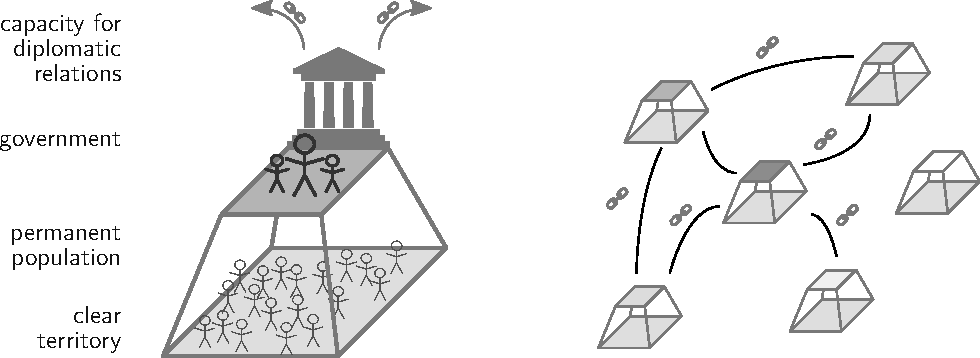
\includegraphics[width=0.9\textwidth]{graphics/basics/countries/decl_const_theory}
  \caption{Declaratory Theory (left) vs. Constitutive Theory (right) of statehood (based on \cite{StateTheory})}
  \label{fig:declaratory_constitutive_theory}
\end{figure}

Both theories have advantages and disadvantages, but the main problems are:
\begin{enumerate}
  \item Following the declarative theory, countries are self-classifying and potentially conflicting entities. The application of this measure would grant Kosovo, the Republic of China and Abkhazia statehood. But this would lead to overlapping territories with Serbia, China and Georgia.
  \item There is no super-national organization that can judge if a country is a country or not. Even the United Nations fail to do so, because their membership requirements prevent states like Kosovo or the Republic of China from becoming members.
\end{enumerate}

Nobody can clearly say if Kosovo, Taiwan or Abkhazia are countries or not -- and if one did, there were people who disagree. This is a big problem for the intended information system, because it is impossible to objectively classify a place as a country or not. Moreover, this section only covers the current countries. 100 years ago these two theories did not exist. It is thus impossible to make a conflict-free decision of what constitutes a country at any point before the \nth{20} century. Moreover, it is also not justifiable because of a lack of jurisdiction. That means, the HGIS developed in this thesis inevitably deals with uncertain information that some parties will disagree with. Its data model cannot perfectly deal with self-classifying data and cannot rely on an objective data source. The system has to contain approaches that deal with these problems.


% subsection declaratory_vs_constitutive_theory (end)

% ------------------------------------------------------------------------------
\subsection{Territory of a Country} % (fold)
\label{sub:territory_of_a_country}

The declaratory theory introduces four main properties of a country. The data model developed in this thesis focuses only on the territory, since it can be easily presented on a map. It can just as well be a complex issue, as it has already been explained for the case of the State of Palestine in section \ref{par:un_observer_states}. In the usual case, the three-dimensional territory of a country consists of the \emph{landmass} it occupies, its \emph{territorial waters} and its \emph{controlled airspace}. This thesis considers only the two-dimensional mapping of the territory on the Earth's surface. It contains land, islands, inland water, river outfalls, and fjords.

The \emph{land territory} is bounded by the country \emph{borders}. A border can be modeled by a set of straight lines between clearly defined \emph{border points}.
A border is either \emph{interior}, when it directly borders the territory of another country on land, or a \emph{coastline} if it borders international water. According to the United Nations, the territory of a country extends in a range of 5 to 20 kilometers into international waters \cite{UNSeaBorders}. This forms the \emph{sea territory} of a county.
An interior border can be either \emph{natural} if it is based on geographical features, e.g.\ a river or a mountain ridge, or \emph{artificial}.
The territory of a country is \emph{continuous} if each point on the territory can be reached by any other point without leaving the territory. Non-continuous territories are usually the case if the country has islands.

\vspace{-0.5em}
\begin{minipage}[t]{0.60\textwidth}

However, there is a special case to be considered:
If a territory is completely surrounded by the territory of exactly one country, it is an \emph{enclave}. On the contrary, an \emph{exclave} is a part of a country's territory that is geographically separated from the main part of the territory. In some cases the exclave of one country is automatically the enclave of another country -- however, if the exclave is surrounded by more than one country, is not an enclave. Enclaves can be nested and form a hierarchy, e.g.\ a \emph{second-order enclave} is an enclave within an enclave
\cite{enclavesexclaves}. \\[-0.6em]

In the example in figure \ref{fig:enclaves_exclaves} ~ $A$ has three exclaves: $A_1$, $A_2$ and $A_3$. Only $A_3$ is also an enclave, within $B$. $E$ is an enclave of $A$. Within $E$, there are two second-order enclaves for $A$, $A_4$ and $A_5$. Inside $A_4$, there is $E_1$, a third-order enclave from the perspective of $A$ and a second-order enclave for $E$. $D$ is the only fully enclaved territory.

\end{minipage}             % N.B. the % is very important
\hspace{0.05\textwidth}    % N.B. this must go in this line, no blank lines !!!
\begin{minipage}[t]{0.35\textwidth}

\vspace{-2em}
\begin{figure}[H]
  \centering
  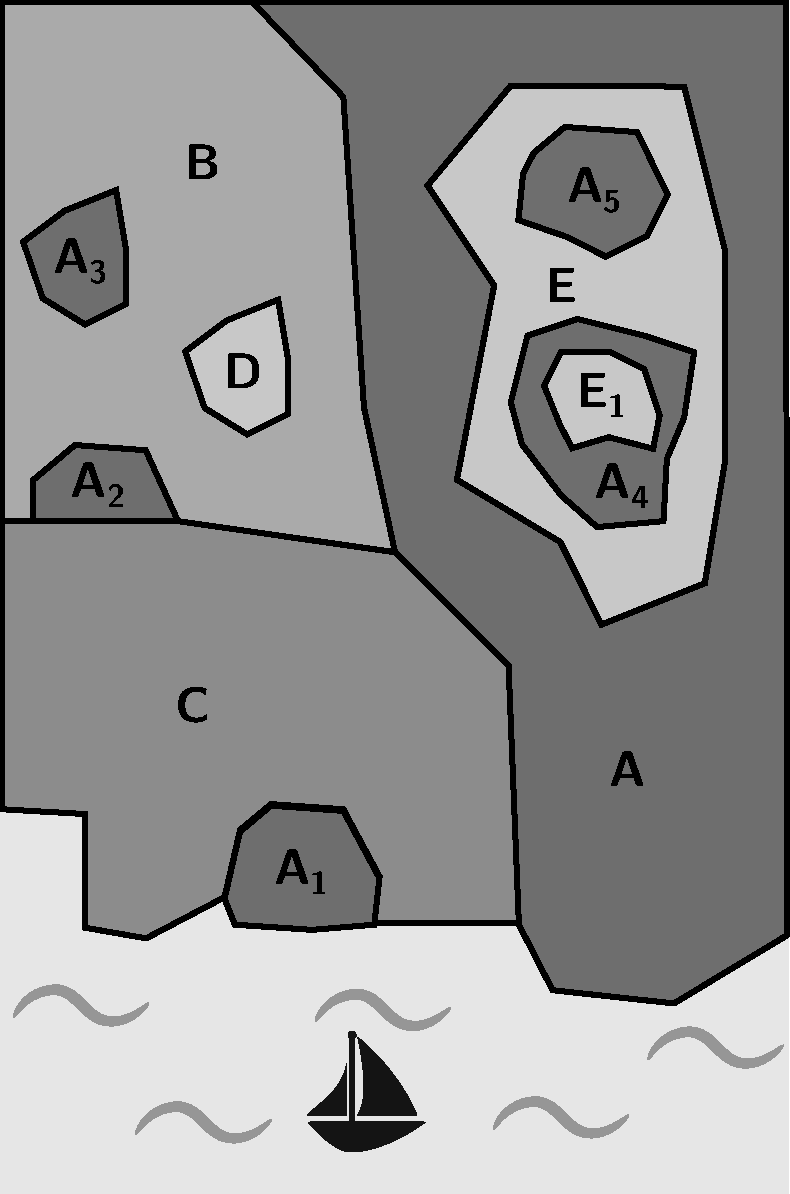
\includegraphics[width=0.9\textwidth]{graphics/basics/countries/enclaves_exclaves}
  \caption{Enclaves and exclaves}
  \small{based on \cite{enclavesexclavesfigure}}
  \label{fig:enclaves_exclaves}
\end{figure}

\end{minipage}    % N.B. the % is very important

Second-order enclaves infrequently appear in the real world, as in the example of Baarle-Nassau and Baarle-Hertog at the border between the Netherlands and Belgium \cite{baarlebaarle}. There are ONLY three countries in the world that are complete enclaves: San Marino, Vatican City and Lesotho.

% subsection territory_of_a_country (end)

% section countries (end)

% ==============================================================================
\section{Historical Geographic Information Systems} % (fold)
\label{sec:historical_geographic_information_systems}

A \emph{system} is an organized structure containing \emph{elements} that are directly or indirectly \emph{related} to each other. At any point in the system's existence there is an \emph{internal state} that changes when it gets influenced by stimuli from the outside \cite{buizdict}. An \emph{information system} is an application that acquires, manages, analyses and presents information \cite{informationSystem}. The terms ``signs'', ``data'', ``information'' and ``knowledge'' are sometimes used interchangeably and there is no coherent definition for any of them. However, all describe different concepts. This explanation seen in figure \ref{fig:information} is based on the work of \cite{datinfwis}.

\begin{figure}[ht]
  \vspace{1em}
  \begin{center}
    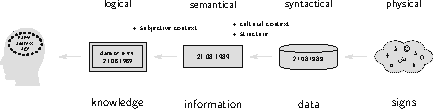
\includegraphics[width=0.9\textwidth]{graphics/basics/hgis/information}
  \end{center}
  \caption{Signs, data, information and knowledge}
  \label{fig:information}
\end{figure}

A \emph{sign} is the physical representation of something in the real world. Since the real world is continuous, literally anything can be seen as a sign, so the set of signs is uncountably infinite.
\emph{Data} is a subset of all possible signs and represents the syntactical level of what an information system deals with. Data itself does not have any meaning, but as soon as it is organized, it becomes \emph{information}.
However, information is sensitive to its cultural context. The string ~\texttt{14.07.1789}~ is useful and understandable for people in countries that use the date format \texttt{DD.MM.YYYY}. However, for people in Belize and the USA this same data might just be a random string of numbers -- it does not have any information.
When a human understands the visualization of information he or she can integrate it into a larger subjective context, the \emph{knowledge} \cite{nake}.
The goal of a visualization is to present the information in a way that it can be transformed into knowledge by the viewer.

If the majority of the information in a system has a spatial relation to the Earth, its surface, its atmosphere or the social structure of its habitation, it is called a \emph{Geographic Information System} (GIS). The data objects in the system are called \emph{geo-objects}
\cite{bolstad2008gis}.
If the information has an additional temporal dimension, e.g.\ via time stamps or time spans, which allow to trace developments of geo-objects, it becomes a \emph{Historical Geographic Information System}
\cite{gregory2014toward}
or alternatively \emph{Spatio-Temporal Information System} (STIS)
\cite{pelekis04stdms}.
HGIS help scholars in \emph{Digital Humanities} to analyze how ``spatial patterns change over time in order to better understand large-scale Earth processes''
\cite{peuquet99}.
Their purpose is to situate ``history in its geographical context and using geographic information to illuminate the past''
\cite{knowles2008placing}.

% ------------------------------------------------------------------------------
\subsection{History vs. Geography} % (fold)
\label{sub:history_vs_geography}

\begin{quoteit}
La Géographie n’est autre chose que l’Histoire dans l’espace, \\
de même que l’Histoire est la Géographie dans le temps. \\[1.0em]
Geography is nothing but History in space, \\
the same way as History is Geography over time.
\end{quoteit}
\hfill \textit{-- Élisée Reclus: ``L'Homme et la Terre'' (1908)}

% - - - - - - - - - - - - - - - - - - - - - - - - - - - - - - - - - - - - - - -
\paragraph{History} % (fold)
\label{par:history}

Like many other fields in the humanities, \emph{history} is ``an ideal field for thinking long and hard about important questions''
\cite{ahaFiveCs}.
It originates from the Greek word \emph{\textIota\textsigma\texttau\textomikron\textrho\textiota\textalpha / historia}: ``finding out, learning through research, narration of what is learned'' \cite{dict}
and it signifies the two main modern usage forms of the term: to research about something and to tell a story. Historians interpret primary sources, such as written documents, photographs or historical maps to explain complex phenomena \cite[pp.4-7]{knowles2008placing}. The main goal of history is to study processes in the past to understand the situation in the present and make reasonable decisions for the future. The American Historical Association has developed the ``five C`s of historical thinking [that] together describe the shared foundations of [the] discipline''\cite{ahaFiveCs}:

\vspace{-1em}
\begin{description} % manipulation of indentation
  \item[Change over time]
  The lives of people, their languages and cultures are continuously changing. One goal of history is to describe these historical changes triggered by historical events. Snapshots in the form of historical maps or historical photography are used to tackle this task.
  \item[Context] The goal is to travel back in time to a moment in the past and recreate the world. Therefor it is crucial to understand the historical context via primary sources.
  \item[Causality]
  The overall goal of each science is to answer the question \emph{why} something is the way it is. Historians want to explain historical events or processs based on evidence. The problem is that history cannot run experiments, because the same conditions cannot be repeated. Therefor historians have to focus on the interpretation of primary sources.
  \item[Contingency]
  Each event has a network of prior conditions, because the world is highly interconnected. A slight change in one prior condition could have led to a completely different outcome of the event and a different state of the world.
  \item[Complexity]
  The intrinsic human need for order conflicts with the contingency of history. It is questionable if all details about events in the world are scientifically explainable.
  This problem is comparable to Heisenbergs uncertainty principle in physics: Physical movements on the macro-level are a direct cause of a set of preconditions, e.g.\ speed, fraction, wind or weight. They are therefore predictable. However, the smallest of all particles are not traceable, their movements are not predictable and therefore their processes not entirely explainable.
\end{description}

% paragraph history (end)

% - - - - - - - - - - - - - - - - - - - - - - - - - - - - - - - - - - - - - - -
\paragraph{Geography} % (fold)
\label{par:geography}

(Greek ~\emph{\textgamma\textepsilon\textomega\textgamma\textrho\textalpha\textphi\textiota\textalpha / geographia}) literally means ``describing the earth''
\cite{dict}.
It is a science that studies the interplay between the landscapes and environments of the Earth (\emph{physical geography}) on the one hand and people, their cultures, societies and economies (\emph{human geography}) on the other. It is an interdisciplinary field between natural and social sciences
\cite{rgsGeography}. Geographical research aims to understand where things are found, why they are there and how they developed over time. It focuses on the interconnectivity between elements of physical and human geography, which gets expressed in Tobler's First Law of Geography: ``Everything is related to everything else, but near things are more related than distant things''
\cite{lawOfGeography}.

Geographers use different techniques to answer their research questions. One important tool is a \emph{map}: a two-dimensional representation of physical, environmental, political, economical or social properties of the Earth. The ``art and science of making maps'' is the field of \emph{cartography} \cite{cartography}.

Since maps visualize a model, they have a natural constraint: ``No map can perfectly replicate the real world, since it inevitably generalizes, abstracts and approximates the complexity of the reality''
\cite[p. 181]{knowles2008placing}.

% paragraph geography (end)

% - - - - - - - - - - - - - - - - - - - - - - - - - - - - - - - - - - - - - - -

\vspace{3em}

\begin{table}[ht]
\begin{center}
\begin{tabular}{p{0px} r c l p{0px}}
    \toprule
    & \emph{Geography}
    & \emph{Aspect}
    & \emph{History}
    & \\
    \midrule
    & Where?
    & Question
    & When?
    & \\

    & Space
    & Dimension
    & Time
    & \\

    & Exact, statistical
    & Character
    & Fuzzy, complex
    & \\

    & Mainly quantitative
    & Research
    & Mainly qualitative
    & \\

    & Spatial proximity of conditions
    & Causal explanation
    & Temporal sequence of events
    & \\

    & Clustering
    & Organization principle
    & Periodization
    & \\

    & Mostly visual (maps)
    & Form of expression
    & Mostly verbal (texts)
    & \\

    & High (GIS)
    & Digitalization potential
    & Low (digital humanities)
    & \\

    \bottomrule
\end{tabular}
\caption{Differences between history and geography \cite[pp. 2-4]{knowles2008placing}}
\label{tab:history_vs_geography}
\end{center}
\end{table}

% subsection history_vs_geography (end)

% ------------------------------------------------------------------------------
\subsection{Geospatial Data} % (fold)
\label{sub:geospatial_data}

A HGIS deals with the temporal development of geo-objects. The geo-objects in this case are the territories of countries. They are usually presented on a \emph{map}. The problem is that the Earth in the real world is three-dimensional and infinitely in detail, but the map is two-dimensional and can only show discrete features. In order to show a country on a map, there are mainly three steps involved:

\begin{enumerate}
  \item Choose a three-dimensional reference surface, an \emph{ellipsoid} or a \emph{spheroid}, that approximates the real shape of the Earth reasonably well.
  \item Define the \emph{geographic coordinate system} to locate each geo-object in using a \emph{geodetic datum}.
  \item Use a \emph{map projection} to show the curved surface of the Earth on a flat two-dimensional map.
\end{enumerate}

% - - - - - - - - - - - - - - - - - - - - - - - - - - - - - - - - - - - - - - -
\paragraph{Reference surface} % (fold)
\label{par:reference_surface}

The shape of the Earth is very complex.
In the Babylonian Empire ($\approx$ 2000-539 B.C.E) the theory of the Earth being a flat disc surrounded by an infinite body of water evolved.
% \footnote{
%   A theory still valid in some southern parts of the United States of America
% }.
The Greek scientists Pythagoras and Aristotle rejected this theory around 340 B.C.E and proved the Earth to be a three-dimensional \emph{spherical} object.
It took almost 2000 years until Sir Isaac Newton reasoned in 1687 that due to the centrifugal forces of the rotating Earth the shape has to be flattened at the poles and is therefore better described as an \emph{ellipsoid}.
However, the model disregards that the surface of the Earth is not smooth but consists of deep oceanic trenches and high mountains. Therefore, the gravitational field of the Earth is not homogeneous either: the actual \emph{mean sea level}, the reference surface for the height of objects, varies from 106 meter below to 85 meter above uniform sea level of the ellipsoid model. These discoveries in the \nth{20} century led to the \emph{geoid}, a physical model of the Earth. The latest and most accurate measurements are the result of the GOCE satellite launched in March 2009 \cite{geoid, geoidESRI}.
However, the geoid is too complex to work with and hence, usually a reference \emph{ellipsoid} is used to approximate the geoid. The ellipsoid is a reference surface with two radii: the polar radius ($r_p$) and the slightly larger equatorial radius ($r_e$) \cite[pp. 69-77]{bolstad2008gis}.

\begin{figure}[H]
  \centering
  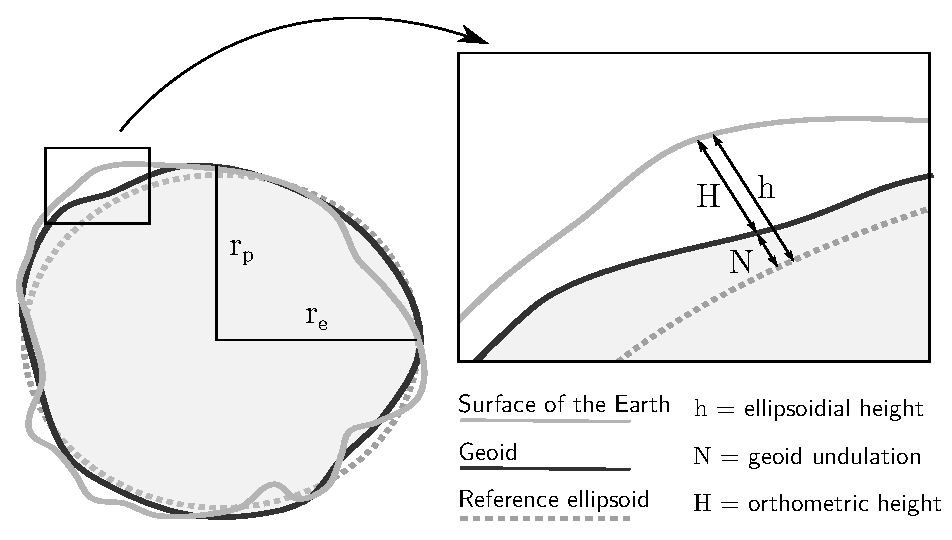
\includegraphics[width=0.9\textwidth]{graphics/basics/hgis/earth_models}
  \caption{Models of the Earth's figure, differences are exaggerated \cite[Fig. 3-6, p. 75]{bolstad2008gis}}
  \label{fig:geoid}
\end{figure}

% paragraph reference_surface (end)

% - - - - - - - - - - - - - - - - - - - - - - - - - - - - - - - - - - - - - - -
\paragraph{Geographic coordinate system} % (fold)
\label{ssub:geographic_coordinate_system}

The reference ellipsoid is expressed in a three-dimensional coordinate system. The \emph{North} and the \emph{South Pole} are defined as the two surface points closest to the Earth's center opposite to each other. The \emph{Equator} is the line equidistant to the two poles and dividing the world in a \emph{Northern} and \emph{Southern Hemisphere}. Additionally, the \emph{Prime Meridian} is defined as the line perpendicular to the Equator, running from the North to the South Pole. Since there are infinitely many lines like this, its definition is arbitrary, but by convention, the line running through Greenwich is used. Based on these two lines, each point in the spherical coordinate system can be unambiguously defined by
\cite[pp. 26-28]{bolstad2008gis}:

\begin{compactenum}
  \item The rotation angle along the Equator, defining its longitude: $\gamma \in [-180\degree ~...~ +180\degree]$
  \item The rotation angle along the Prime Meridian, defining its latitude: $\phi \in{=} [-90\degree ~...~ +90\degree]$
  \item The distance to the origin: $r > 0$
\end{compactenum}

\begin{figure}[ht]
  \vspace{0.5em}
  \centering
  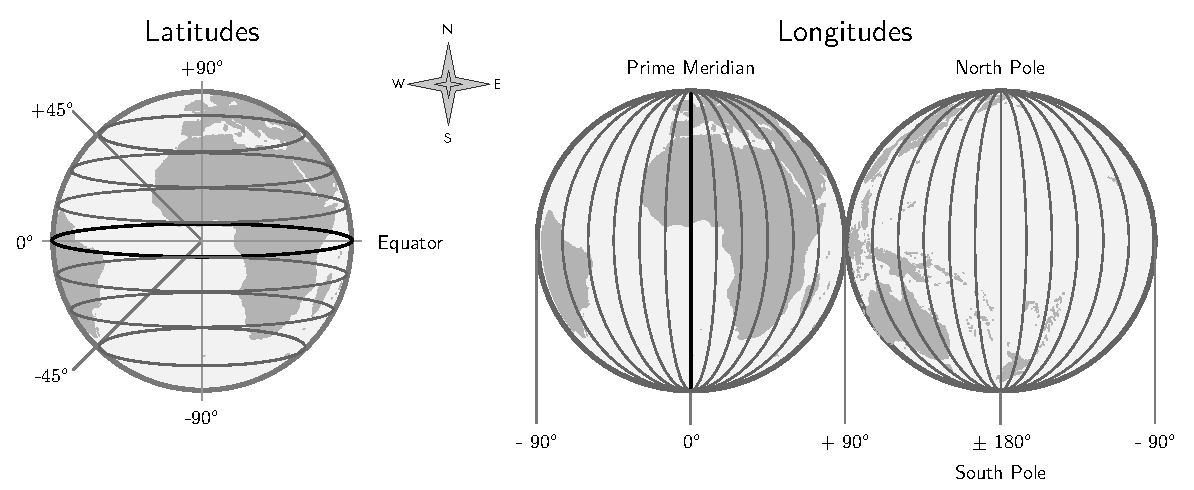
\includegraphics[width=0.9\textwidth]{graphics/basics/hgis/geo_coordinates}
  \caption{Geographic coordinates using latitude and longitude}
  \label{fig:geo-coordinates}
\end{figure}

Lines of constant latitude are running horizontally and are called \emph{parallels}, lines of constant longitude in vertical direction are \emph{meridians}. All parallels are circles with their center on the axis between the poles. No two parallels intersect. The longest parallel is the Equator (0\degree~latitude). All meridians have the same length. Geographic coordinates are usually recorded either in degree-minutes-second (\texttt{DMS}, e.g.\ \texttt{50\degree~58' 22''}) or in decimal degree (\texttt{DD}, e.g.\ \texttt{50.973}) notation
\cite[pp. 30, 79]{bolstad2008gis}.

The geometric ellipsoid aims to fit the physical geoid as good as possible. The \emph{geodetic datum} is a geographic coordinate system, usually based on an ellipsoid, that defined a set of reference points that relate to the geoid. There are a lot of different geodetic datums, because they can be very accurate in one region of the world, but inaccurate in another. The same geographic coordinates in two different geodetic datums define two different points on Earth. Therefore, it is essential to know the geodetic datum of the coordinates \cite[p. 80]{bolstad2008gis}.
The \emph{World Geodetic System 1984 (WGS84)} is a model that found worldwide acceptance and is used in all major web-based mapping services like \emph{OpenStreetMap} and in the GPS unit of major mobile devices.

% paragraph geodetic_datum (end)

% - - - - - - - - - - - - - - - - - - - - - - - - - - - - - - - - - - - - - - -
\paragraph{Map projections} % (fold)
\label{par:map_projections}

In the last step, the surface of the three-dimensional ellipsoid has to be projected onto a two-dimensional map that can be printed on paper or visualized on a computer screen.
Because the surface of the ellipsoid is curved, some features of the Earth will be distorted on the map: An \emph{equal-area projection} preserves the area sizes of features on the map, whereas a \emph{conformal projection} preserves angles and the shapes of objects. Every map projection that is area-preserving distorts shapes at the same time, and each shape-preserving map distorts areas to some degree. There is no perfect map projection that presents all features of the real world correctly \cite{mapProjectionGeokov}.
A compromise between preserving areas and shapes is the \emph{Robinson projection}: it is neither conformal, nor equal-area, but provides a reasonable trade-off between both properties.


\begin{figure}[H]
  \centering
  \begin{tabular}{c c}
    \begin{subfigure}{0.5\textwidth}
      \centering
      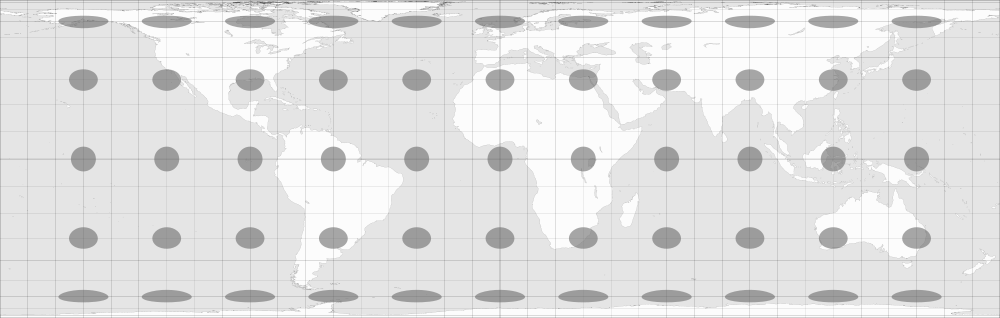
\includegraphics[width=0.9\linewidth]{graphics/basics/hgis/projection_distortion_lambert.png}
      \caption{Equal-area Lambert projection}
    \end{subfigure}
    &
    \multirow{2}{*}{
      \begin{subfigure}{0.4\textwidth}
        \vspace{-2.8em}
        \centering
        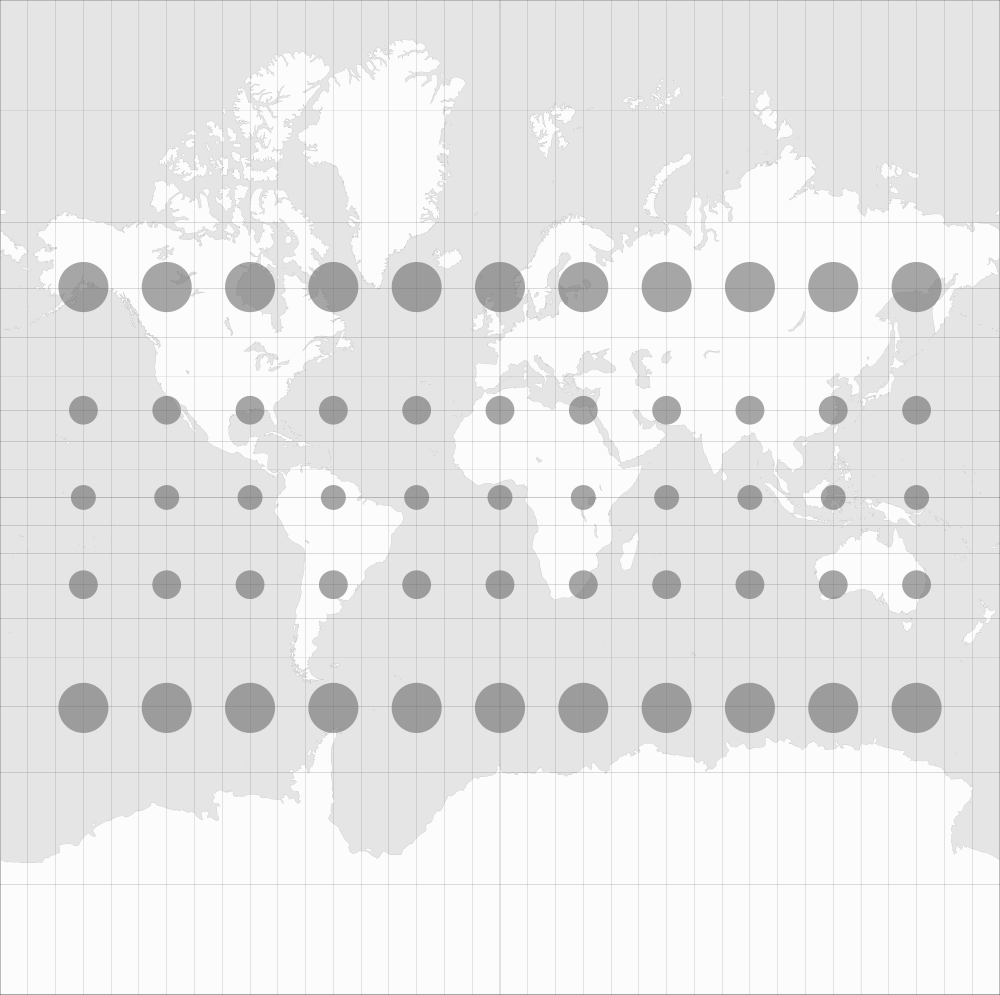
\includegraphics[width=0.9\linewidth]{graphics/basics/hgis/projection_distortion_mercator.png}
        \caption{Conformal Mercator projection}
        \label{fig:mercator}
      \end{subfigure}
    } \\
    \begin{subfigure}{0.5\textwidth}
      \vspace{1em}
      \centering
      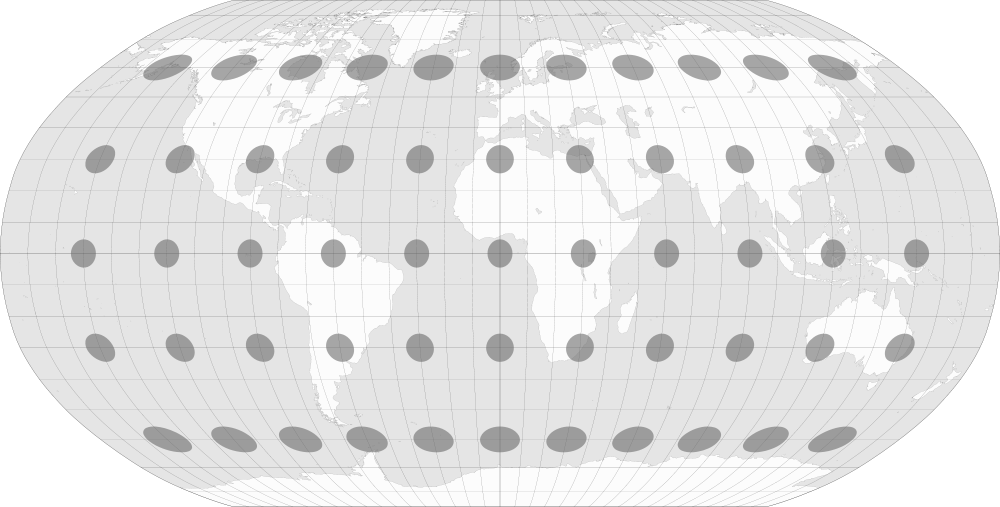
\includegraphics[width=0.9\linewidth]{graphics/basics/hgis/projection_distortion_robinson.png}
      \caption{Compromise Robinson projection}
    \end{subfigure}
    & \\
  \end{tabular}
  \caption{Comparison between different map projections, based on \cite{mapProjections}}
  \label{fig:map_projections}
\end{figure}

% paragraph map_projections (end)

% - - - - - - - - - - - - - - - - - - - - - - - - - - - - - - - - - - - - - - -
\paragraph{Digital maps} % (fold)
\label{par:maps}

A map in a HGIS is structured according to the \emph{layer} principle: Each layer is a transparent film showing one specific aspect, e.g.\ a physical layer for landmasses or water and a political layer for international borders and names of countries. The layers are interchangeable and can be shown and hidden. A \emph{legend} including the scale bar and north arrow should explain all symbols used on the map and give orientation. Interactive maps may have additional control options for panning and zooming, switching map layers on and off or changing the color scheme of the map
\cite[pp. 159-166]{bolstad2008gis}.

An example of such interactive map services is \emph{Leaflet.js}, ``an open-source JavaScript library for mobile-friendly interactive maps''
\footnote{
  \textit{Leaflet - JavaScript library for interactive maps},
  URL: \url{http://leafletjs.com/},
  accessed on: 02.11.2015
}.
It is used in the implementation of this this thesis. A leaflet map is embedded in a HTML document on the client-side of a web-based information system. Additionally, the user can include own map layers, symbols and markers on that map. Leaflet uses a conformal Mercator projection, comparable to figure \ref{fig:mercator}, also known as \emph{Web Mercator}.

% - - - - - - - - - - - - - - - - - - - - - - - - - - - - - - - - - - - - - - -
\paragraph{Vector Model} % (fold)
\label{ssub:vector_model}

The real world is infinite in detail, but storage in a computer is finite. In order to model continuous geographical phenomena in an information system, a relevant subset of them should be sampled to create discrete spatial data. It can be represented either in a raster or vector model. In the vector model each spatial object is expressed by three basic geometric primitives.

\begin{figure}[H]
  \vspace{1em}
  \centering
  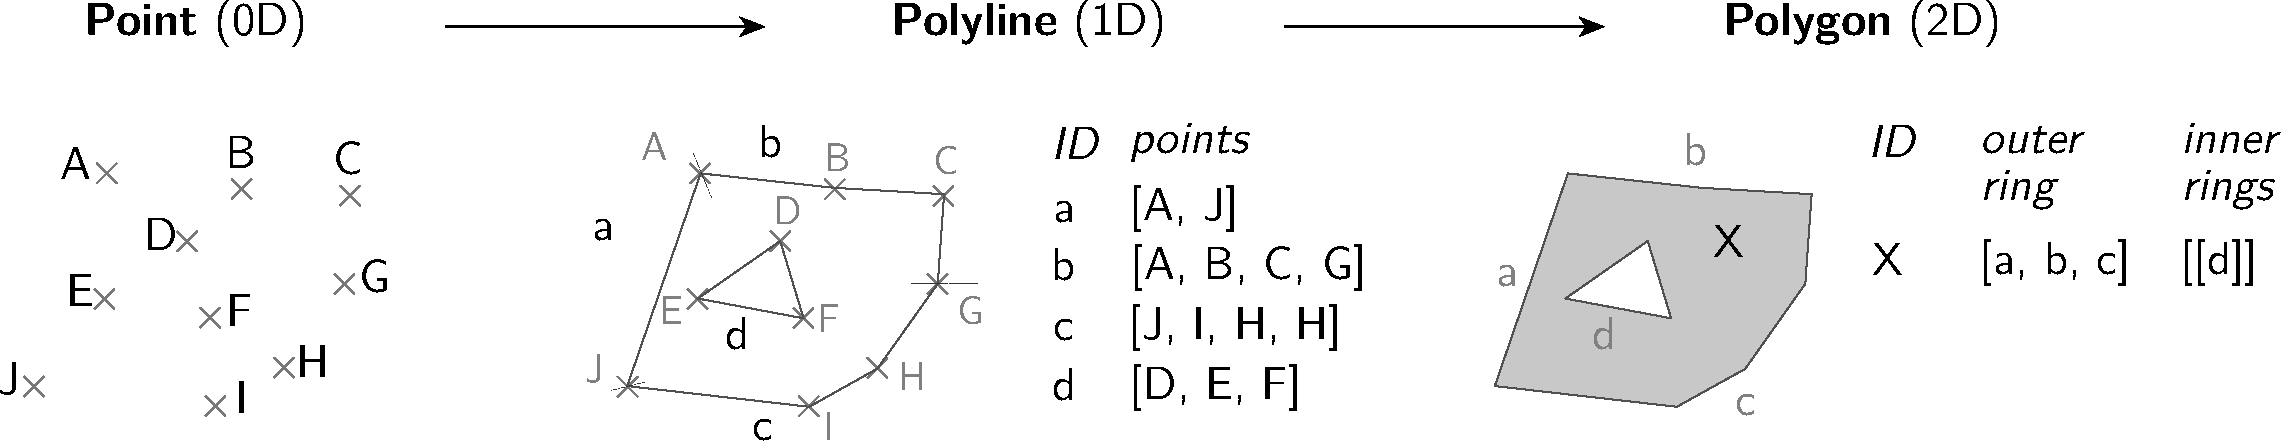
\includegraphics[width=0.9\textwidth]{graphics/basics/hgis/geometric_primitives}
  \caption{The basic geometric primitives point, polyline and polygon}
  \label{fig:geometric_primitives}
\end{figure}

\begin{enumerate}
  \item[0D] A \emph{point} is the fundamental object in vector geometry. It has no dimension and is only defined by its position, specified in geographic coordinates. A point is independent from all others.
  \item[1D] A \emph{polyline} is an ordered set of at least two points. The outermost ones are the start and end point.
  \item[2D] A \emph{polygon} describes a closed surface and is constructed by one set of polylines forming a closed \emph{outer ring}. Additionally, there can be multiple sets of polylines as \emph{inner ring} representing holes in the polygon. If the polygon has no inner rings it is a \emph{simple} polygon, otherwise it is \emph{weakly simple}. If it is even self-intersecting, as shown in figure \ref{fig:polygon_properties}, the polygon is \emph{complex}. \emph{Polypolygons} represent multiple separate polygons belonging to one logical entity \cite{polygons}.
\end{enumerate}

\begin{figure}[H]
  \centering
  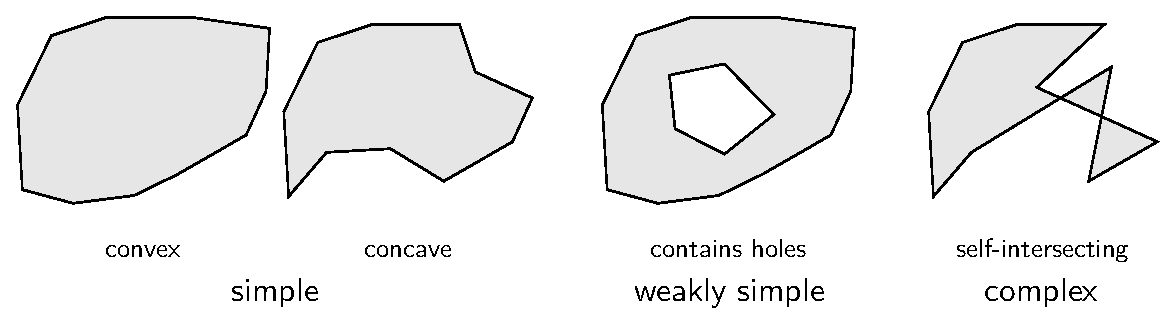
\includegraphics[width=0.9\textwidth]{graphics/basics/hgis/polygon_properties}
  \caption{Types of polygons}
  \label{fig:polygon_properties}
\end{figure}

There are mainly three Boolean \emph{set operations} that can be performed on two polygons: \emph{Union}, \emph{intersection} and \emph{difference}. A \emph{symmetric difference} is a combination of two differences. Their definition is visualized in figure \ref{fig:polygon_operations}.
If multiple polygons are unified at once, it is a \emph{cascaded union}
\cite{bolstad2008gis}.

\begin{figure}[ht]
  \centering
  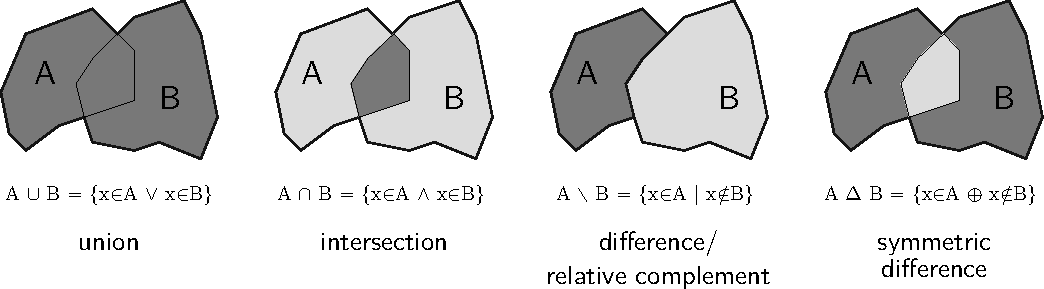
\includegraphics[width=0.9\textwidth]{graphics/basics/hgis/polygon_operations}
  \caption{Boolean set operations on polygons, the dark gray area is the result of the operation}
  \label{fig:polygon_operations}
\end{figure}

Common file types for geospatial vector data are the open format GeoJSON
\footnote{
  \emph{GeoJSON},
  IETF GeoJSON Working Group,
  URL: \url{http://geojson.org/},
  accessed on: 30.10.2015
}
%, Scalable Vector Graphics (\texttt{.svg})
% \footnote{
%   \emph{W3C SVG Working Group},
%   IETF Geographic JSON Working Group,
%   URL: \url{http://www.w3.org/Graphics/SVG/},
%   accessed on: 30.10.2015
% }
or ESRI Shapefiles
\footnote{
  \emph{ESRI Shapefile Technical Description},
  ESRI White Paper, July 1998,
  URL: \url{http://www.esri.com/library/whitepapers/pdfs/shapefile.pdf},
  accessed on: 30.10.2015
}.

% paragraph vector_model (end)

% subsection geospatial_data (end)

% ------------------------------------------------------------------------------
\subsection{Temporal Data} % (fold)
\label{sub:temporal_data}

Time is an abstract concept that ``can be perceived only by its effects''
\cite[p. 27]{Langran1989timeingis}.
Many philosophers and scientists have developed models to deal with time. For this thesis, the model needs to be appropriate to represent time in a historical sense and in interplay with geographical space. A popular model is \emph{Cartographic Time}, where time is seen as the ``fourth cartographic dimension''
\cite[p. 28]{Langran1989timeingis}.
Unlike space, time knows only one dimension. Relative to one point, time has two directions: historically \emph{forward} into the future and \emph{backward} into the past.
The topological relationship between two points in time $t_1$ and $t_2$ is straightforward, because there are only three different order relations: $t_1 < t_2$, $t_1 > t_2$ and $t_1 = t_2$.

% - - - - - - - - - - - - - - - - - - - - - - - - - - - - - - - - - - - - - - -
\paragraph{Types of Time} % (fold)
\label{par:types_of_time}

Whereas space is represented by geo-objects, time may be represented by discrete \emph{events} and continuous \emph{processes}. Events can happen at a certain \emph{point in time} or like processes in a \emph{time interval} or \emph{time period}, defined by two time stamps
\cite[chapter 2, pp. 47-49]{solana2014spatio}.
The \emph{Taxonomic Model of Time} classifies time also by its \emph{nature} or \emph{time order}
\cite{frank98typesoftime}:
a consecutive development on the time axis, defined by start and end, defines \emph{linear time}. In contrast, \emph{cyclic time} has no predefined order and events reoccur on a regular cyclic basis. Two further types, \emph{branching time} and \emph{multi-dimensional time}, are more complex and not relevant for this thesis.


% paragraph types_of_time (end)

% - - - - - - - - - - - - - - - - - - - - - - - - - - - - - - - - - - - - - - -
\paragraph{Timelines} % (fold)
\label{sub:timelines}

In contrast to space, time does not have an intrinsic representation. However, the most common form of visualizing cyclic time is on a cyclic display, e.g.\ a  clock. Linear time is mostly visualized on a \emph{timeline}. The purpose of it is to show events as points in time or processes as time intervals in chronological order. A timeline shows additional time markers on a certain date to support orientation. The position of an event on the timeline is described by its date using a reasonable sampling unit like century, year or day
\cite[p. 32]{Langran1989timeingis}.
A timeline uses a certain time scale:

\begin{itemize}
  \item On a \emph{linear} timeline, the distance between any two points in time is directly proportional to their actual temporal distance.
  \item A \emph{logarithmic} timeline uses a logarithmic function to scale the depicted time. There is a reference point on the timeline, e.g.\ the center. Similar to linear timelines, the farther away a point is from the reference point, the farther away it is positioned on the timeline. However, the distance between this point and the reference point does not increase linearly -- events that are further away appear less far. This time scale accounts for logarithmic human perception: Given two events $A$ and $B$, whereas $A$ happened 20 years ago and $B$ ten years ago. The perceived temporal distance between $A$ and $B$ is smaller than the distance between $B$ and today, although the absolute distance is the same
  \cite{logorlinear}.
  \item A the scale of a timeline can also be \emph{irregular}, e.g.\ to get the same distance between events on the timeline. This is particularly useful if the events are not distributed homogeneously.
\end{itemize}

\begin{figure}[ht]
  \centering
  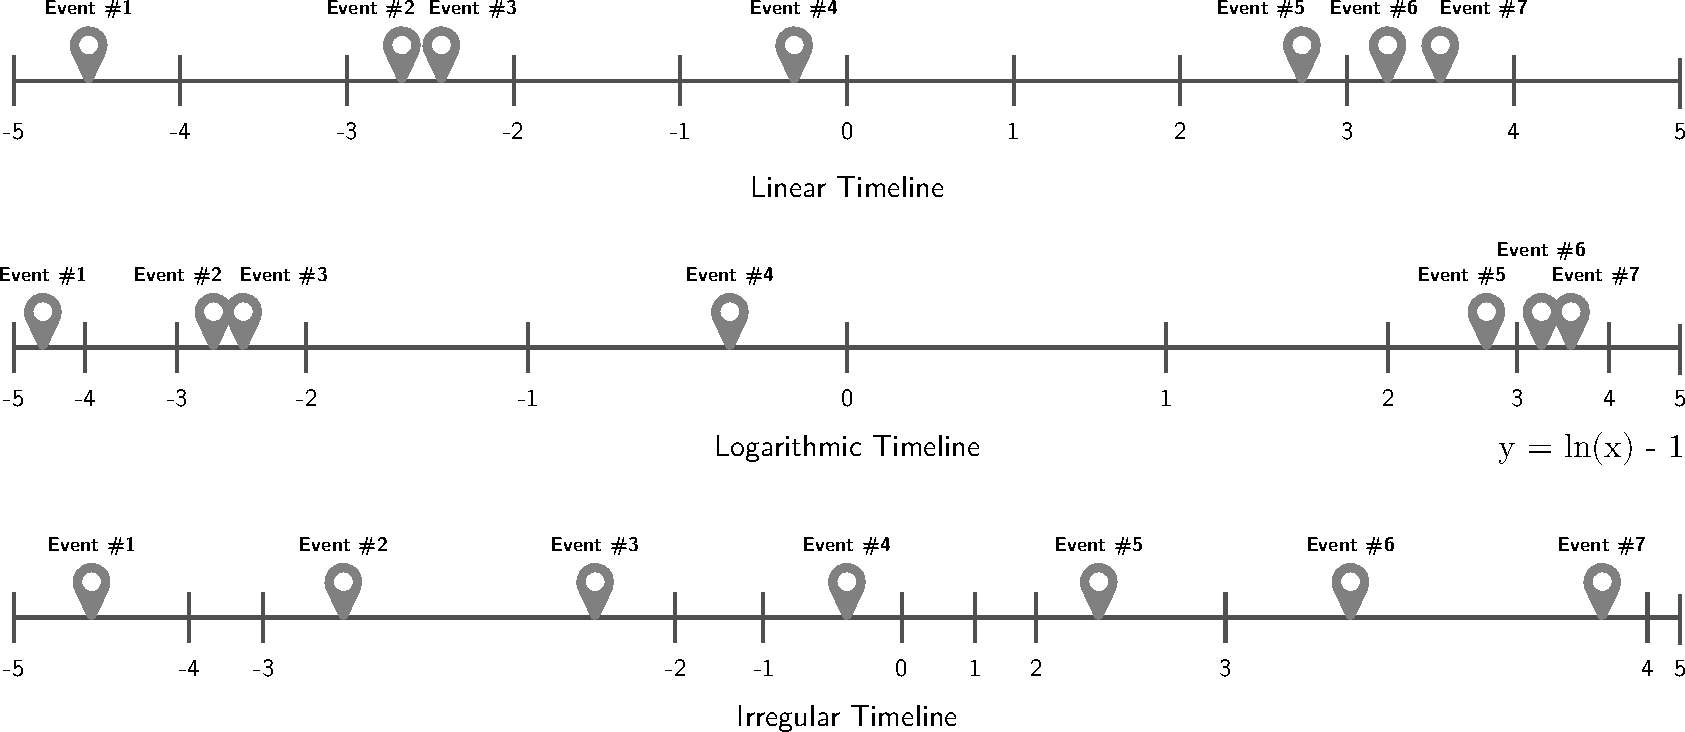
\includegraphics[width=0.9\textwidth]{graphics/basics/hgis/timelines}
  \caption{Comparison between a linear, a logarithmic and an irregular timeline}
  \label{fig:timelines}
\end{figure}

% subsection temporal_data (end)

% ------------------------------------------------------------------------------
\subsection{Existing Applications} % (fold)
\label{sub:applications}

``Today, operational temporal GIS does not exist''
\cite[p. 5]{raza12}.
This quote nicely summarizes the state of the art in this field. The main reasons are ``the complexity of integrating space and time and the lack of standards''
\cite[p. 5]{raza12}.

However, there are numerous HGIS projects for one specific research question. A large collection can be found in \cite{knowles2008placing} and \cite{gregory2014toward}.
One example related to the topic of this thesis is the \emph{Great Britain Historical GIS Project} (GBHGIS)
\footnote{
  \textit{Great Britain Historical Geographical Information System (GBHGIS)},
  Ian Gregory \& Humphrey R. Southall, University of Portsmouth, since 1994,
  URL: \url{http://www.port.ac.uk/research/gbhgis/},
  accessed on: 02.11.2015
}.
It maps statistical data on historical territorial units of the United Kingdom (UK) using \emph{aerial interpolation}
\cite{aerialInterpolation}.
One purpose is for example to analyze net migration in the districts of the UK. The data is collected by the \emph{British Ordnance Survey} that automatically detects spatial changes to the geography of the United Kingdom using aerial photography \cite{ordnanceSurvey}.
The \emph{National Historical Geographic Information System} (NHGIS)
\footnote{
  \textit{Welcome to NHGIS},
  Minnesota Population Center, University of Minnesota,
  since 2007,
  URL: \url{https://www.nhgis.org/},
  accessed on: 02.11.2015
}
provides the digital boundaries of the United States of America and census data for each year since 1790. While the data in the system is extensive, the interface to analyze and use the data is very cumbersome to use.
% A tutorial is necessary to go through the incredibly complex selection process. To download data, a user has to register, receive an email with a link to download a compressed file which has to be decompressed and then loaded into a GIS software to be visualized.

HGIS are not widely accepted in the humanities. One reason is the nature of the qualitative historical research: historic sources are subjective and biased, their content may be fuzzy and they are definitely incomplete. Therefore, the knowledge that can be extracted from a source bears the integral problem of \emph{uncertainty}. Information systems on the other hand have a logical architecture and try to be as precise and accurate as possible. Analysis is based on mathematical functions -- an information system is quantitative in its entire nature
\cite[p. 2]{knowles2008placing}.


% subsection applications (end)

% ------------------------------------------------------------------------------
\subsection{Data Sources} % (fold)
\label{sub:data_sources}

The HGIS developed in this thesis requires historical data about countries, their names, borders, historical events and their introduced changes to countries. There are a lot of free and open sources for geographic data about the current countries, their names and borders. One of the most exhaustive collections of geographic data in the public domain is hosted by Natural Earth
\footnote{
  \textit{Natural Earth},
  URL: \url{http://www.naturalearthdata.com/downloads/},
  accessed on: 30.10.2015
}.
There is physical data, e.g.\ coastlines and rivers, and cultural data, e.g.\ political borders and cities available.
Data about historical countries and events are not as straightforward to acquire, because of the mostly qualitative nature of historical research (see section \ref{sub:history_vs_geography}). The most exhaustive free and open source of historical data is \emph{Wikipedia} and their article categories, e.g.\ \texttt{armistices} or \texttt{treaties}
\footnote{
  \textit{Category:Treaties},
  Wikipedia, the free encyclopedia,\\
  URL: \url{https://en.wikipedia.org/wiki/Category:Treaties},
  accessed on: 13.05.2016
}.
All sorts of historical events can be found. Some information is structured in information boxes, e.g.\ some historical treaties contain a name, location, a signature and an effect date. Particularly interesting for this thesis are articles about historical countries
\footnote{
  \textit{List of former sovereign states},
  Wikipedia, the free encyclopedia,
  URL: \url{https://en.wikipedia.org/wiki/List_of_former_sovereign_states},
  accessed on: 13.05.2016
},
because they contain the name and important meta information, e.g.\ their historical successors and predecessors.

The creation of an open-source HGIS on the basis of Wikipedia would be a huge project with significant impact on open education -- however, it would also be a big challenge: not all historical countries and events that are required to model the history of the world are available on Wikipedia. It is also inconsistent, because not all articles are structured, especially not to those of events that actually have an influence on a territorial change of a country, e.g.\ a border agreement. Retrieving, parsing and processing this information is challenging.
Further consideration must be given to accuracy and quality of information in Wikipedia, due to their open source nature.
Overall, using Wikipedia as a data source for this thesis is not feasible, but this is subject to further research.

% - - - - - - - - - - - - - - - - - - - - - - - - - - - - - - - - - - - - - - -
\paragraph{Historical maps} % (fold)
\label{par:historical_map}

The most problematic data to acquire are historical borders of countries. There is no primary data source for that, so the most promising way is the extraction of a border from a historical map. They can be found on Wikipedia as well, or in historical map collections, e.g.\ \emph{OldMapsOnline}
\footnote{
  \textit{Old Maps Online},
  URL: \url{http://www.oldmapsonline.org/},
  accessed on: 13.05.2016
}.
The project is developed ``out of a love of history and heritage of old maps'' and stores about 400 000 historical maps.
There are five steps to retrieve the points of a border in geographic coordinates from a historical map. This process was developed in a preceding \emph{HiBo -- Historical Borders} project \cite{hibo}.

\begin{enumerate}
  \item \textbf{Digitization}: If the map is on paper, it has to be scanned in the best possible quality. The result is a raster graphic.
  \item \textbf{Georeferencing}: The historical map has to fit as good as possible on the reference map. This requires a manual definition of a set of reference points which are used to transform the map into the geographic coordinate system. This process is error-prone, especially if the projection of the historical map is not known and the map itself is not accurate
  \cite{knowles2002past}.
  The outcome is a rectified and resampled raster graphic in which each pixel is assigned a geographic coordinate.
  \item \textbf{Preprocessing}: The raster image has to be processed so that the desired border stands out and can be traced in the next step. This happens via greyscale conversion, thresholding or the Canny Edge Detector to find edges in a raster image \cite{canny}. This results in a monochrome graphic in which the desired border must be uninterrupted and clearly be seen.
  \item \textbf{Line detection}: By selecting a start and an end point of the border, the line gets traced automatically. This step vectorizes one particular feature, a borderline, from the raster graphic and produces a polyline in geographic coordinates.
  \item \textbf{Postprocessing}: In the last step, the polyline can be adapted. The line can be simplified to reduce unnatural artifacts and the position of border points can be manually edited. The final output of the whole process is a polyline whose points are expressed in the geographic coordinate system. This can further be used as a border of a historic country.
\end{enumerate}

\begin{figure}[ht]
  \centering
  \begin{subfigure}{0.48\textwidth}
    \centering
    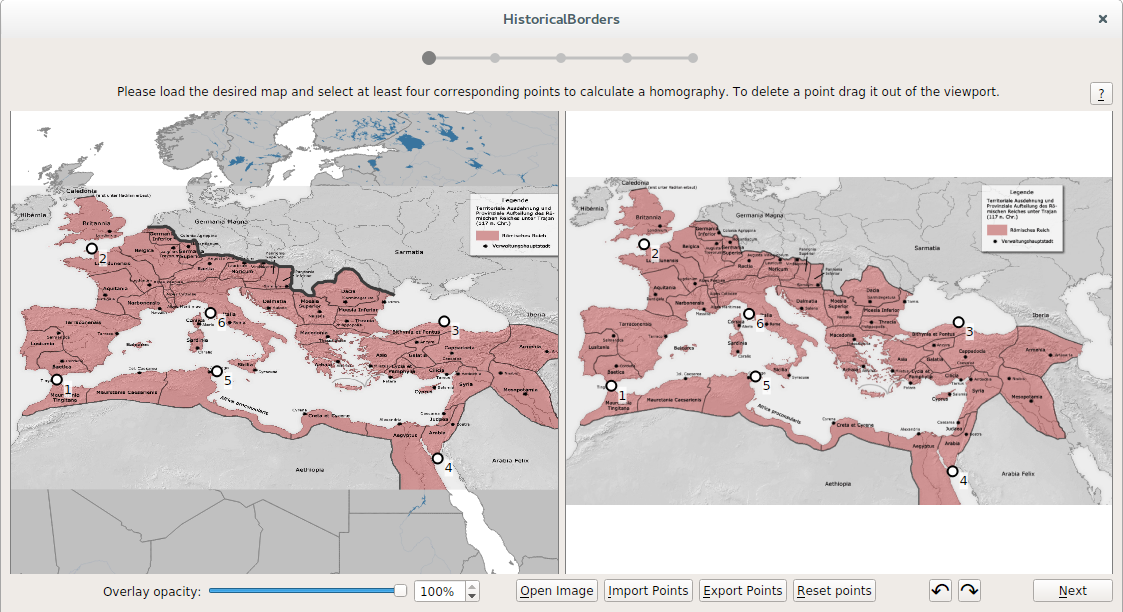
\includegraphics[width=0.95\linewidth]{graphics/basics/hgis/hibo1.png}
    \caption{Georeferencing}
  \end{subfigure}
  \begin{subfigure}{0.48\textwidth}
    \centering
    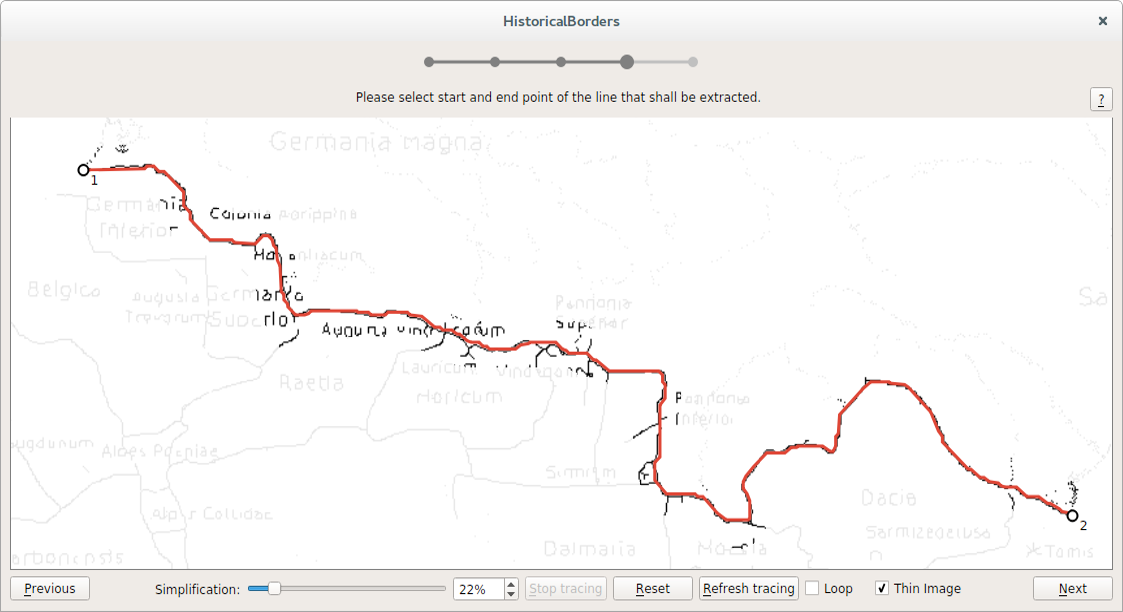
\includegraphics[width=0.95\linewidth]{graphics/basics/hgis/hibo2.png}
    \caption{Semi-automatic digitizing}
  \end{subfigure}
  \caption{Semi-automatic extraction of a border from a map of the Roman Empire \cite{hibo}}
  \vspace{2em} % wtf ?!?
  \label{fig:hibo}
\end{figure}


% paragraph historical_map (end)

% subsection data_sources (end)

% section historical_geographic_information_systems (end)

% ==============================================================================

\section{Spatio-Temporal Data Models} % (fold)
\label{sec:spatio_temporal_data_models}

\begin{quoteit}
  ``Geography differs from geometry because \\
  in geography, space is indivisibly coupled with time''
\end{quoteit}
\hfill -- Don Parkes \& Nigel Thrift (1980)

A data model abstracts a part of the real world, identifies the most essential elements and their relation to each other. Historical Geographic Information Systems use spatio-temporal data models to explain the historical development of geographic phenomena. Based on the theory of the \emph{Triadic Framework}, three components are involved: space (3 dimensions), time (1 dimension) and attribute (1 dimension for each). Each of these dimensions can change independently from each other
\cite[p. 53]{ott2001time}.
However, in order to trace spatial and attribute changes over time, the dimensions have to be related to each other. Spatio-temporal data models establish these relations.

Throughout the lifetime of a geo-object, it appears at some point in time, can undergo several changes and can disappear at some other point. \emph{Discrete changes} are based on the idea of a \emph{state machine}. At any point in the lifetime, an object is in a certain state. It stays there until an event occurs that suddenly changes the object into a new state, e.g.\ the German Reunification in 1990 unified East and West Germany to present-day Germany. On the contrary, an object can gradually change according to a \emph{continuous process}, e.g.\ the change of the coastlines due to the sea level rise
\cite{peuquet99}.

In the previous 30 years many spatio-temporal data models were developed. The basis for each of them is the concept of \emph{Time Geography}
\cite{haegerstrand1970}:
There is an orthogonal relationship between time and space. At each point in time an object is at exactly one location. The models can be classified by their organizing dimension: In \emph{location-based} models time is an attribute of a geo-object. In contrast, \emph{event-based} approaches focus on events and processes that change geo-objects. This section introduces different spatio-temporal data models that are relevant for this thesis.

% \emph{Entity-based} models represent geo-objects as own entities. Spatial changes over time are related to these entities, but they are not attributes and therefore independent.

% The visualization of time can be separate from the spatial dimension, according to the Triadic Framework, e.g.\ with a timeline. In another approach, space and time can also be coupled and displayed in the same presentation display, e.g.\ in a space-time cube \cite{haegerstrand1970}.

% ------------------------------------------------------------------------------
\subsection{Snapshot Model} % (fold)
\label{sub:snapshot_model}

As already introduced in section \ref{sec:problem_domain}, the \emph{Snapshot model} stores the full state of all geo-objects at certain points in time $t_i$ in a snapshot. It is one of the simplest, oldest and most frequently used spatio-temporal models despite its severe disadvantages
\cite{Langran1988frameworktgis}.

\begin{figure}[H]
  \vspace{1em}
  \centering
  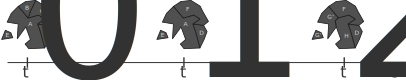
\includegraphics[width=0.9\textwidth]{graphics/basics/stdm/snapshot_model}
  \caption{The Snapshot model \cite{Langran1988frameworktgis}}
  \label{fig:snapshot_model}
\end{figure}

For all other points $t \neq t_i$ that are not covered by a snapshot, it is impossible to retrieve the state of the system, because the data model does not record any changes. This is an integral problem of the model and cannot be solved. Therefore, it is unsuitable for the domain of this thesis. The original model is also redundant, because objects that have not changed from one snapshot to the next one are duplicated. However, improvements were made to tackle this problem, e.g.\ \cite{armenakis92}.

% subsection snapshot_model (end)

% ------------------------------------------------------------------------------
\subsection{Simple Time-Stamping} % (fold)
\label{sub:simple_time_stamping}

The simplest approach to trace the history of a geo-object is to assign a period of existence to it. This happens by adding two attributes: at the \emph{start date} $t_{start}$ the object is created and at the \emph{end date} $t_{end}$ it is deleted. If an object still exists it gets a special value, e.g.\ \texttt{NOW}, as its end date
\cite{hunter90timestamping}.

\begin{figure}[H]
  \vspace{1em}
  \centering
  
\includegraphics[width=0.9\textwidth]{graphics/basics/stdm/simple_time_stamping}
  \caption{The Simple Time-Stamping method \cite{hunter90timestamping}}
  \label{fig:simple_time_stamping}
\end{figure}

The \emph{Simple Time-Stamping} method is also location-based and tracks discrete changes of objects. Given full and consistent information, the state of the system at an arbitrary point $t_i$ can be retrieved: each geo-object for which ~$t_{start} \leq t_i < t_{end}$~ is active, all others are inactive. However, this retrieval is cumbersome, because without efficient data structures every time the date changes, it has to be checked for each geo-object if its state has changed.

Another problem of the model is that it does not allow for tracing historical relations between geo-objects. As an example, at $t_1$ $B$ and $C$ end and $F$ starts. Visually, $F$ is a successor of $B$ and $C$, but this historical relationship cannot be deducted directly from the model. This shortcoming can be resolved by adding a reference to the predecessor and the successor of the object.

This model alone is not suitable for the domain of this thesis, because it is impossible to say what exactly has happened at a certain point in time. Given the example above, it is unclear if two objects unified to a new one ($B+C \to F$) or if two are successors ($B \to F$) and one just stops to exist ($C \to \emptyset$). The model is also redundant: if a geo-object replaces another one ($B \to F$), then $t_{end}$ of $B$ is the same as the $t_{start}$ of $F$
\cite[p. 46-47]{solana2014spatio}.

% subsection simple_time_stamping (end)

% ------------------------------------------------------------------------------
\subsection{Event-Based Spatio-Temporal Data Model} % (fold)
\label{sub:event_based_spatio_temporal_data_model}

A time-based approach addresses exactly these shortcomings. They explicitly represent events or processes in the data model and associate all objects that change according to them. One example of this approach is the \emph{Event-Based Spatio-Temporal Data Model} (ESTDM) for geospatial raster data \cite{peuquet95}.
At one defined point in time $t_b$, a snapshot gets stored. This \emph{base map} contains the current state of the map, i.e.\ the current value of each raster cell \texttt{(x,y)}. From that moment on, the system stores events that change the values of certain cells. Such an event has a time stamp (\texttt{t}) and a list of components associated with it. A component represents a new value (\texttt{v}) and knows which raster cells (\texttt{x}, \texttt{y}) change their value to \texttt{v}.

The method uses the following data structures: a header file contains information about the thematic domain, a pointer to the base map and to the first and last element of the event list. This doubly-linked list stores all events chronologically. Therefore, each event knows its preceding and succeeding event. If the time stamp of an event is reached, all its components are executed, i.e.\ the relevant raster cells change their value. The system follows the \texttt{next} pointer to know which event is waiting to be executed next. Since a change is relative to the previous change and not to the base map, change tracking is efficient.

The concept of the ESTDM suits the problem domain really well. A historical event changes the geometry of certain objects suddenly. The model explicitly represents these discrete changes. However, it does not work for vector data. The authors have explicitly stated that ``the design of such a [vector-based] model is not seen as a straightforward task'', because of the problem ``how to maintain the integrity of spatial topology as it changes [...] The solution will require a more complex definition of components within individual events''
\cite[p. 21]{peuquet95}.

\begin{figure}[H]
  \vspace{1em}
  \centering
  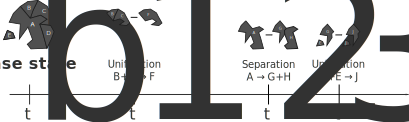
\includegraphics[width=0.9\textwidth]{graphics/basics/stdm/event-based_spatio-temporal_data_model}
  \caption{An example for an event-based spatio-temporal data model for vector data}
  \label{fig:event-based_spatio-temporal_data_model}
\end{figure}

% Also, just like the Simple Time-Stamping method, this model is only suitable for discrete but not for gradual changes. This problem is solved in the \emph{ObjectOriented geomorph} model by \cite{raperlivingstone95}.

% subsection event_based_spatio_temporal_data_model (end)

% ------------------------------------------------------------------------------
\subsection{Three-Domain Model} % (fold)
\label{sub:three_domain_model}

An event-based STDM for vector geometry including lines and polygons has to answer the following questions: What uniquely identifies a geo-object? What kind of spatial, topological and attribute changes can happen to an object? Which of these maintain the identity and which create a new object? This problem is addressed in the \emph{Three-Domain} model by \cite{yuan96threedomain, yuan96temporal}. The model is based on abstract entities that represent a spatio-temporal object. It handles the three domains identity, space and time separately:
\begin{itemize}
  \item The \emph{semantic domain} holds an entity uniquely identifiable. An object in this domain corresponds to a human concept, e.g.\ a ``country''.
  % It handles attributes of the area, but not the spatial and temporal properties.
  \item The \emph{spatial domain} represents the geospatial object in vector format representing the country.
  \item The \emph{temporal domain} stores all temporal objects, e.g.\ time stamps of a historical event.
\end{itemize}

The model is not specific, but rather a general abstract framework to handle space, time and identity. This makes the model very flexible, e.g.\ it can handle discrete and continuous changes, relative and absolute time, world and database time. One limitation is that it only traces spatial attributes over time. In an alternative model by \cite{claramunt95timeingis}, the \emph{thematic domain} is added to fully describe a spatio-temporal object and trace also non-spatial attributes that can change over time, e.g.\ the name of a country. Since countries, their territories and attributes can change independently over time, the data model used in this thesis will be organized according to the Three-Domain model.

% subsection three_domain_model (end)

% ------------------------------------------------------------------------------
\subsection{History Graph Model} % (fold)
\label{sub:history_graph_model}

Most of the data models introduced so far cover only static changes of geo-objects. \cite{renolen96} identified three different types of temporal behavior of changing objects:
\begin{compactitem}
  \item Dynamic objects that change continuously.
  \item Static objects that change according to events with duration (processes).
  \item Static objects that change according to sudden events.
\end{compactitem}

Based on this observation a data model that can handle all three kinds of temporal behavior was developed: the \emph{History Graph} model. It manages objects and events separately from each other. An object can only be in three different states:
\begin{enumerate}
  \item An object is \emph{static}, if it currently does not change. This is called an \emph{object version}. The version has an interval associated to it representing the duration of the object version, until it changes next time. If the object is dynamic and changes continuously, the duration is zero.
  \item If an object is currently \emph{changing}, it is in an \emph{object transition}. The transition also has an associated interval with a duration of zero for a sudden change. Additionally, a transition links the relevant objects to each other to establish a historical predecessor-successor-relationship.
  \item An object that is currently not active, is \emph{ceased} and not visible on the map.
\end{enumerate}

\begin{figure}[H]
  \centering
  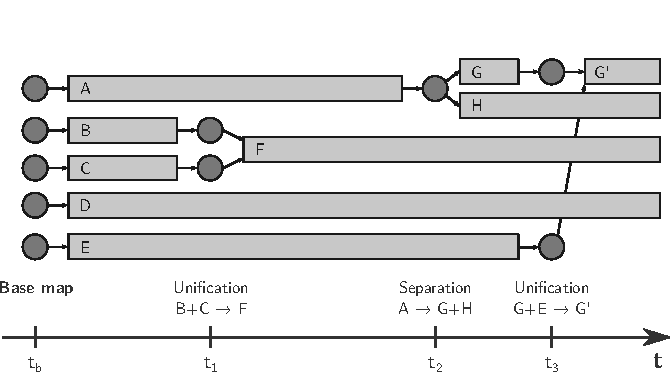
\includegraphics[width=0.60\textwidth]{graphics/basics/stdm/history_graph_model}
  \caption{The History Graph model}
  \label{fig:history_graph_model}
\end{figure}

The history of a geo-object is a chronologically ordered set of versions and transitions, that can be visualized in a graph like the one in figure \ref{fig:history_graph_model}.
The model defines six basic types of temporal changes that can happen. They can be seen in figure \ref{fig:history_graph_changes}:

\begin{compactitem}
  \item \textbf{Creation}:           A new object is created.
  \item \textbf{Alteration}:         A property of an object, e.g.\ its geometry, changes.
  \item \textbf{Cessation}:          An object ceases to exist.
  \item \textbf{Reincarnation}:      An object that has previously been deleted is recreated.
  \item \textbf{Split/Deduction}:    An object is divided into multiple new objects, or at least one new object is deducted from an existing one.
  \item \textbf{Merge/Annexation}:   Multiple objects are unified to a new object, or at least one object is annexed to another object.
\end{compactitem}

\begin{figure}[ht]
  \vspace{1em}
  \centering
  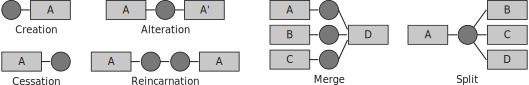
\includegraphics[width=0.9\textwidth]{graphics/basics/stdm/history_graph_changes}
  \caption{Types of changes in the History Graph model}
  \label{fig:history_graph_changes}
\end{figure}

The History Graph model can be seen as an extension to the ESTDM. It combines the advantages of event-based and location-based STDM and supports discrete and continuous changes. The main improvement is that the historical development of a geo-object can be directly derived from the model, because objects are linked to their predecessors and successors -- the History Graph model can tell a story. This is the reason why this model is particularly suitable for this thesis.

% subsection history_graph_model (end)

\vspace{1em}
Other popular spatio-temporal data models that are not covered in this work, because they were not seen as relevant for the domain, including the \emph{Space-Time Composite} model, the \emph{Grid model} and the \emph{Amendment Vector model}. Overviews about these and other spatio-temporal data models can be found in \cite{zhao11}, \cite{pelekis04stdms} and \cite{peuquet99}.

% section spatio_tempora_data_models (end)


% ------------------------------------------------------------------------------
\subsection{Spatio-Temporal Databases} % (fold)
\label{sub:spatio_temporal_databases}

The data models that have been presented in this section have to be converted to a database model in order to implement them as the management component of the information system. A \emph{Database Management System} (DBMS) is a software system for the administration of data, mainly storage and retrieval. There are mainly two types of DBMS: The oldest and most common ones are \emph{Relational DBMS}. \emph{Object-Oriented DBMS} were developed to adapt concepts of object-oriented programming into the database world. The combination of both approaches are \emph{Object-Relational DBMS}.

% - - - - - - - - - - - - - - - - - - - - - - - - - - - - - - - - - - - - - - -
\paragraph{Relational DBMS} % (fold)
\label{par:relational_dbms}

RDBMS are built upon the concept of \emph{entities} and \emph{relations}. An entity represents an object in the real world with a set of \emph{attributes} and attribute values of a simple data type (e.g.\ \texttt{string} or \texttt{int}). Entities are represented in a table with one row for each \emph{tuple} and one column for each attribute. An entity has one attribute that unambiguously identifies each tuple, the \emph{primary key}, usually a contiguous number. Entities can be related to each other in three different kind of relations:
\begin{compactenum}
  \item[\texttt{1:1}] Direct attributional relation, e.g.\ one country has one capital and vice versa.
  \item[\texttt{1:n}] One-to-many relation, e.g.\ one country can have many cities, but each of those cities can belong to only one country.
  \item[\texttt{m:n}] Many-to-many relation, e.g.\ one country can have many rivers, but each river can also flow through multiple countries.
\end{compactenum}

The first RDBM developed was \emph{Oracle}, released in 1979 \cite{oracleDB}. Since then, the concept has been established as the state-of-the-art for databases. An example for a RDBMS used for web-based systems is \emph{MySQL}, the ``world's most popular open source database''
\footnote{
  \emph{MySQL :: About MySQL},
  URL: \url{https://www.mysql.com/about/},
  accessed on: 31.10.2015
}.

% paragraph relational_dbms (end)

% - - - - - - - - - - - - - - - - - - - - - - - - - - - - - - - - - - - - - - -
\paragraph{Object-oriented DBMS} % (fold)
\label{par:object_oriented_dbms}

One problem with RDBMS is that attributes can only have simple data types. Developers using object-oriented programming need to map the objects used in the application to tuples in the relational database and vice versa. This process can be cumbersome. OODBMS solve this problem by adopting the concepts of object-oriented programming for database management purposes
\cite{oodbms}.
The following and many more object-oriented principles are supported:

\begin{itemize}
  \item \emph{Classes} are structured representation of things in the real world of the same kind of properties, e.g.\ a country with a name and a territory. Classes in OODBMS relate to entities in RDBMS.
  \item An \emph{object} is an instance of a class, one specific thing with defined properties, e.g.\ a country with its territory. This relates to a tuple in RDBMS.
  \begin{itemize}
    \item The \emph{attributes} of an object cannot just be of a simple data type, but also instances of other classes, e.g.\ \texttt{country.territory} can be a \texttt{polypolygon} object.
    \item Objects also have \emph{methods} that can be called to do something with the object, e.g.\ \texttt{territory.getCenter()} returns the geometrical center of the polypolygon.
  \end{itemize}
  \item The internal state of an object cannot be accessed from the outside. Methods are the only way to interact with an object. This is called \emph{encapsulation} and maintains control over what can be done to and with an object and prevents corruption.
  \item According to the concept of \emph{inheritance}, classes can be hierarchically structured, whereas the attributes and the methods of a \emph{base class} are inherited to its \emph{derived class}. As an example, an \texttt{Area} has a \texttt{name}, a \texttt{territory} and the method \texttt{getArea()} associated to it. A \texttt{Country} can be derived from the \texttt{Area}, inheriting both attributes and the method. Additionally, it can get an attribute \texttt{head\_of\_state}, which is specific to \texttt{Country}, but not to \texttt{Area}. The class \texttt{Ocean} can just as well be derived from \texttt{Area}, but it does not need a \texttt{head\_of\_state}.
  % \item An associated concept is \emph{polymorphism}: The same function can be called on different objects and the return value will be of the same type. However, internally it might be calculated differently. As an example, consider the classes \texttt{Polygon} and \texttt{Polypolygon}, both inherited the method \texttt{getArea()} from their base class \texttt{Geometry}. Whereas a polygon calculates its area directly based on its geometry, a polypolygon internally calles the function \texttt{getArea()} on all its associated polygons and sums up their areas.
\end{itemize}

% Vice versa, There is no need for an additional query language

% paragraph object_oriented_dbms (end)

% - - - - - - - - - - - - - - - - - - - - - - - - - - - - - - - - - - - - - - -
\paragraph{Object-relational DBMS} % (fold)
\label{par:object_relational_dbms}

ORDBMS combine the advantages of both worlds. Internally, the established and efficient relational database is used for the data storage. The database model and the interaction with the data happens in an object-oriented way while supporting all of the concepts mentioned in the previous subsection \ref{par:object_oriented_dbms}. The most popular ORDBMS example for web-based systems is \emph{PostgreSQL}, ``the world's most advanced open source database''
\footnote{
  \emph{PostgreSQL:},
  The world's most advanced open source database,
  URL: \url{http://www.postgresql.org/},
  accessed on: 31.10.2015
}.

% paragraph object_relational_dbms (end)


% - - - - - - - - - - - - - - - - - - - - - - - - - - - - - - - - - - - - - - -
\paragraph{Spatio-temporal database models} % (fold)
\label{par:spatio_temporal_database_models}

The spatio-temporal data models discussed in section \ref{sec:spatio_temporal_data_models} need to be implemented in a relational, object-oriented or object-relational database management system. While the details depend on the data model, there are common concepts and issues that have to be addressed. When storing time related data, it is important to distinguish between the time at which something happened in reality (\emph{world time}) and the time it was stored in the database (\emph{database time}). For this thesis, only world time is relevant.

Object-oriented concepts are more appropriate than relational ones, because of the complex nature of spatio-temporal data \cite[section 3.9]{pelekis04stdms}. One of the first implementations was the \emph{spatio-temporal object} combining geometrical and bi-temporal properties in one object \cite{worboys90stdm}. A similar approach by \cite{raza12} is the \emph{Spatio-Temporal Data Type} (STT): Time is not considered an attribute of space, but a separate class. They are aggregated in the \texttt{SpatioTemporal} class, using both spatial and bi-temporal attributes. The model also provides spatio-temporal operators, e.g.\ \texttt{STT\_intersects} returns \texttt{true} if two \texttt{SpatioTemporal} objects intersect in time and space, i.e.\ their geometries intersect and the time intervals in which they are active overlap. These operators are very helpful when analyzing spatio-temporal data or checking for data integrity.

Finally, a severe issue is \emph{version management}. Given a database model that stores geo-objects that are created, updated and destroyed by events. Events cannot only be appended to the end of the timeline, but also in between. This is called a \emph{retrospective update}. It might create conflicting situations, e.g.\ if it deletes a geo-object that would be manipulated in a later event. The question is how to maintain data integrity on insertion, update and deletion from a spatio-temporal database? This issue has to be addressed using formal logic for temporal reasoning
\cite[section 6]{peuquet99}.

% paragraph spatio_temporal_database_models (end)

% subsection spatio_temporal_databases (end)


% ==============================================================================
\section{HistoGlobe} % (fold)
\label{sec:histoglobe}

\begin{quoteit}
  Imagine a globe that you can rotate and see from all sides. \\
  Imagine a timeline which you can scroll to any point in time. \\
  Imagine you can see how the world changes when you move the timeline: \\
  Country borders shift, peoples migrate on the planet or kingdoms give way for democracies. \\[0.5em]
  This is HistoGlobe, a revolution of teaching and learning of history!
\end{quoteit}

HistoGlobe is a web-based HGIS that aims to visualize the history of the Earth on a globe with a timeline. It shows historical events and geopolitical changes. The goal is to provide a freely accessible open-source tool for a

\begin{compactitem}
  \item better \emph{understanding} of history for learners,
  \item more appropriate \emph{presentation} of history for teachers and
  \item interesting \emph{exploration} of history for scholars.
\end{compactitem}

The HistoGlobe project was founded in Weimar in 2010 and has evolved since then from a single student project via a tech-startup with up to 15 contributors to an academic project for the sake of research for geography, history and computer science. The current prototype of HistoGlobe was developed for students in school to understand German, European and World history since World War I with a focus on the time of the Cold War. The prototype can be seen on \texttt{http://histoglobe.com}.

\begin{figure}[ht]
  \vspace{1em}
  \centering
  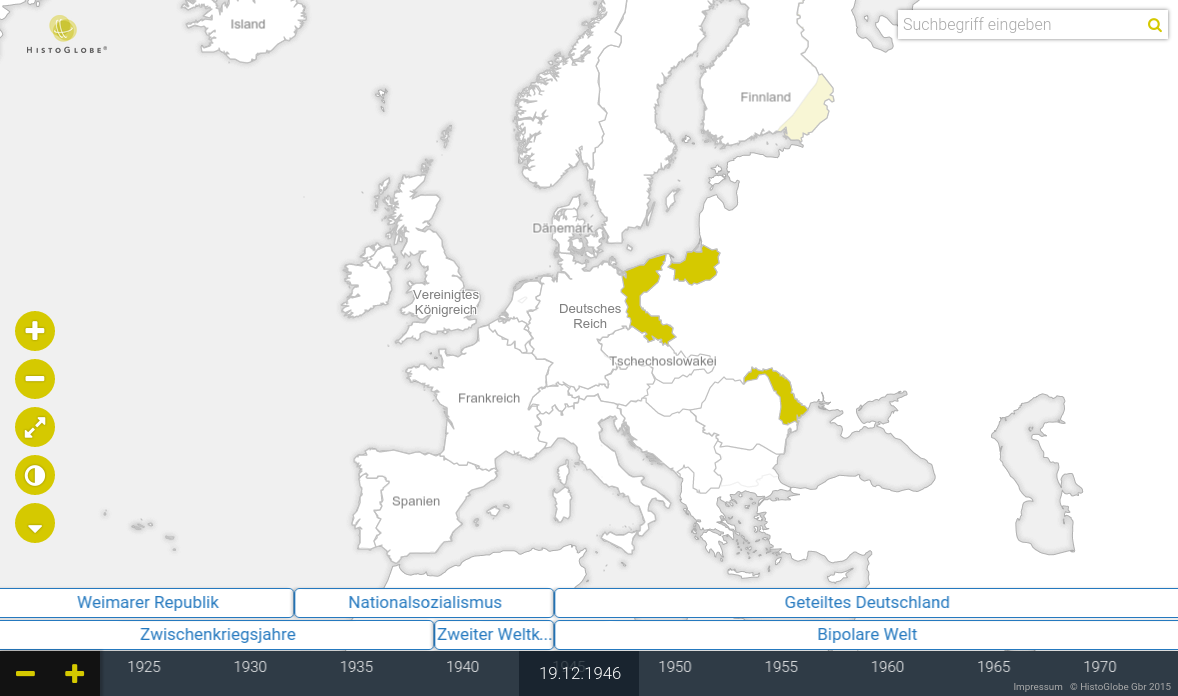
\includegraphics[width=0.9\textwidth]{graphics/basics/histoglobe/school_project}
  \caption{The HistoGlobe school project (April 2015)}
  \label{fig:histoglobe_school}
\end{figure}

Figure \ref{fig:histoglobe_school} shows the user interface of HistoGlobe: a 2D map, a timeline and control buttons for both. Addtionally, a topic bar extends the timeline showing historical periods in German and world history and a search bar for finding historical events. HistoGlobe is built upon a module system for interface components. The map can be exchanged with a globe, control buttons can be switched on and off or additional visualization approaches, e.g.\ for the History Graph introduced in section \ref{sub:history_graph_model}, can be added. The idea is that the components are independent from each other, e.g.\ exchanging the map with a globe has no effect on the timeline or the control buttons. The main problem of HistoGlobe is the data: editing historical information about countries and events is very cumbersome due to a complex domain and a lack of a back-end. Therefore, there is very little data in the system.

% section histoglobe (end)

% ==============================================================================
\vspace{2.0em}

This chapter introduced the problem domain of Historical Geographic Information Systems for the history of countries. Also existing spatio-temporal data models, their advantages and disadvantages have been discussed. The purpose of this thesis is to develop a model for managing the historical developments of countries in time and space. This model will combine some of these approaches and also consider complex cases due to the uncertain nature of historical research. It will be implemented as the foundation of HistoGlobe. Additionally, an editor for historical data is to be developed as a new HistoGlobe module to enable users to edit the course of history directly on the map. The next chapter will present the development process for the data model and the user interface.

% chapter bascis (end)
